\documentclass[conference]{IEEEtran}
\usepackage[table]{xcolor}


\usepackage{tikz, calc}
\usepackage{cite}
\usepackage{hyperref}
\usepackage{url}
\usepackage{graphicx}
% \usepackage{svg}
\usepackage{subcaption}
\usepackage{float}
\usepackage{booktabs}
\usepackage{listings}
\lstset{
  basicstyle=\ttfamily,
  columns=fullflexible,
  frame=single,
  breaklines=true,
  postbreak=\mbox{\textcolor{red}{$\hookrightarrow$}\space},
}
\usepackage{pifont}% http://ctan.org/pkg/pifont
\newcommand{\cmark}{\checkmark}%
\newcommand{\xmark}{\ding{55}}%


\graphicspath{{./figures/}}
%\graphicspath{{./tmp_figures/}}

% \let\marginpar\oldmarginpar
\setlength{\marginparwidth}{5cm}
% \newcommand{\Bnote}[1]{\textbf{[Boaz: #1]}}
\usepackage[colorinlistoftodos,prependcaption, textwidth=3cm]{todonotes}



\title{
Statistical Theory\\
Chess Dataset Analysis
}

% Authors must not appear in the submitted version. They should be hidden
% as long as the \iclrfinalcopy macro remains commented out below.
% Non-anonymous submissions will be rejected without review.

\author{
   \IEEEauthorblockN{Dor Boker, Itamar Nakar}
   \IEEEauthorblockA{
      I.D: 209271279 , 325829000\\
      Email: dorboker@gmail.com, itamar.nakar@gmail.com
   }
}

\newcommand{\fix}{\marginpar{FIX}}
\newcommand{\new}{\marginpar{NEW}}

\listfiles
\begin{document}


\maketitle

\section{Introduction}
Chess is one of humanity's oldest board games \cite{chesswiki}, played by two players on an $8\times8$ grid. Each player, controlling 16 pieces of their color, aims to checkmate the opponent's King, making it impossible for the King to escape capture. Unlike many games, chess does not involve luck or hidden information; the outcome is determined solely by the players' knowledge, strategy, and analytical skills.

The length of a chess match is influenced by several factors, including the players' skill levels, strategic choices, and in-game dynamics. In this project, we investigate the relationship between player ratings and the duration of chess matches, aiming to determine whether higher-rated players tend to play shorter or longer games. In addition to player ratings, we examine other variables that may impact match length, such as opening strategies, game outcomes (win, loss, draw), and time controls.

Our dataset \cite{dataset} comprises 19,113 games from Lichess, an online chess platform, each described by 16 features. The most relevant features to our analysis are: \begin{itemize} \item \textbf{Turns}: A positive integer representing the length of the game, where one turn includes a move by both White and Black. \item \textbf{ELO Rating}: A system that quantifies player skill, widely used by FIDE and online chess platforms \cite{ELO}, which we use to assess its correlation with match length. \item \textbf{Time Controls}: Competitive games are categorized into four main time control classes: Bullet, Blitz, Rapid, and Classical, based on initial clock times and increments \cite{time}. \item \textbf{Winner and Victory Status}: These columns capture whether White or Black won and the method of victory (checkmate, resignation, draw). \end{itemize} Through statistical analysis, we aim to understand how these factors influence the duration of chess matches and to provide insights into the relationship between skill level and game dynamics. 

\section{Results}
\subsection{Data Transformation}

To optimize the quality of our analysis, we undertook a cleaning process to remove entries that could distort or obscure meaningful insights from the dataset. Below are the key transformations:

\begin{itemize}
    \item \textbf{Uncompetitive Games}: Games marked as casual or non-competitive were excluded. Such games may not reflect players' full effort or strategic depth, and are thus not representative of a standard chess match.   
 
    \item \textbf{Elo Adjustments}: New players are initially assigned an Elo rating of 1500, which can skew the distribution of player strength. To mitigate this, each player's rating was updated to reflect their most recent Elo score within the dataset.
\end{itemize}

\begin{figure}[H]
    \centering
    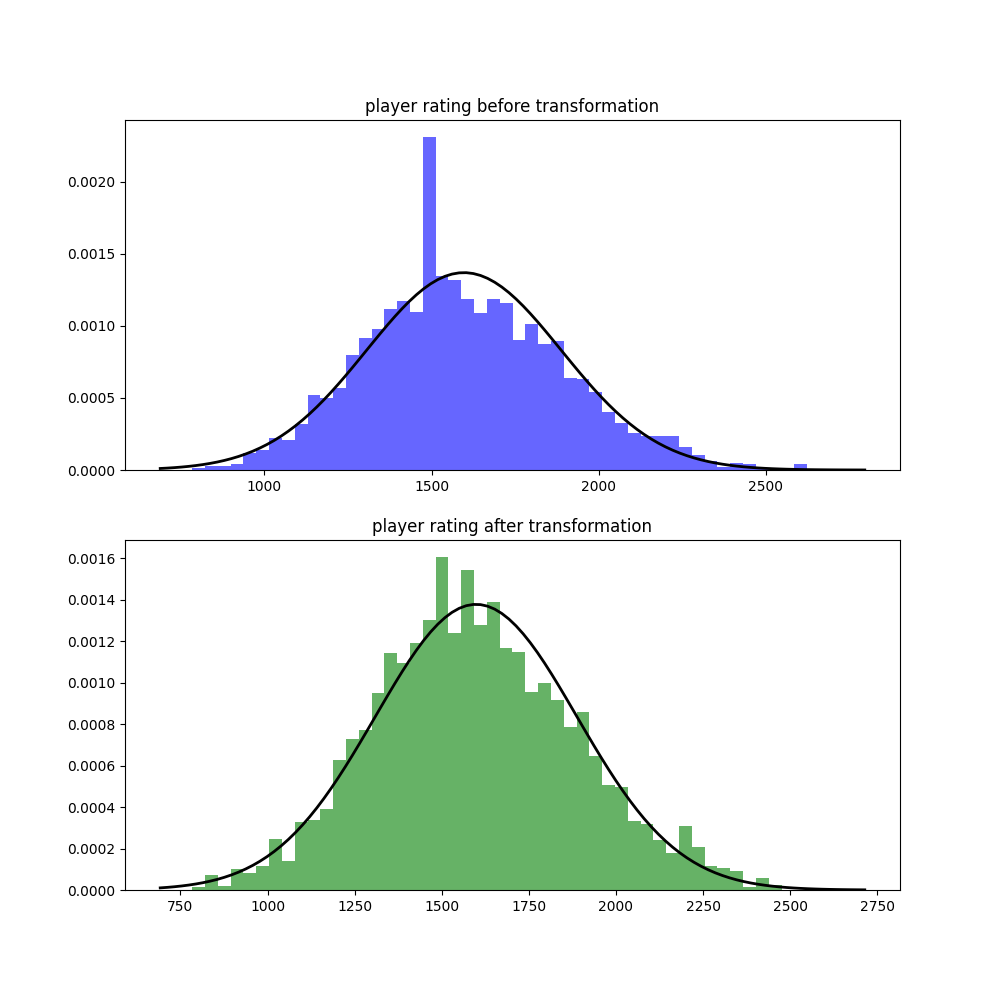
\includegraphics[width=0.8\linewidth]{transformation_plot.png}
    \caption{Transformation's effected on Rating and Turns}
    \label{fig:transformation_plot}
\end{figure}


After these trasformations, we are left with 16,155 games which we will now begin to analyze.

\subsection{Rating Distribution}
The distribution of player ratings in the dataset initially resembles a normal distribution with a peak around the mean. However, this peak diminishes when games involving unrated players are excluded, bringing the distribution closer to normality. This is illustrated in Figure~\ref{fig:transformation_plot}. Additionally, the QQ plot (Figure~\ref{fig:rating_qq}) supports the similarity between the player rating distribution and a normal distribution, albeit with deviations at the tails, which are exacerbated by the QQ plot's sensitivity to deviations at the tail.

\begin{figure}[H]
    \centering
    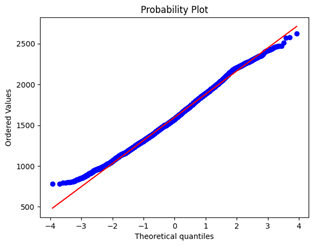
\includegraphics[width=0.8\linewidth]{ratingqq.png}
    \caption{Quantile - Quantile plot of white player rating in relation to normal distribution}
    \label{fig:rating_qq}
\end{figure}


\subsubsection*{Kolmogorov-Smirnov (KS) Test for Normality}
We applied the Kolmogorov-Smirnov (KS) test to evaluate whether the player rating distribution follows a normal distribution. The test returned a p-value of \(8.9649 \times 10^{-13}\), which is significantly lower than the threshold of \(0.03\) for a confidence level of 97\%, thus rejecting the null hypothesis that the rating distribution is normally distributed. However, when the test was performed on a random 10\% sample of player ratings, the p-value increased to 0.49, meaning we could not reject the null hypothesis at that sample size. This result indicates that while the entire population does not fit a normal distribution, smaller samples may approximate normality \cite{kssample}.


\subsection{Relations Between Features}
Analyzing the dataset’s correlation matrix reveals linear relationships between certain features. For example, there is a weak positive correlation between the players' average rating and game length. There are also weak negative correlations between the number of turns and both the absolute difference in player ratings and the 'winner' variable, where 'winner' is numerized as 0 for draws and 1 for games with a winner. From these correlations, we can tentatively conclude that:
\begin{itemize}
    \item Games involving more skilled players tend to last longer.
 
    \item Games with a larger skill gap between players may end faster.

    \item Draws tend to draw out longer then desicive games.
\end{itemize}

\begin{figure}[H]
    \centering
    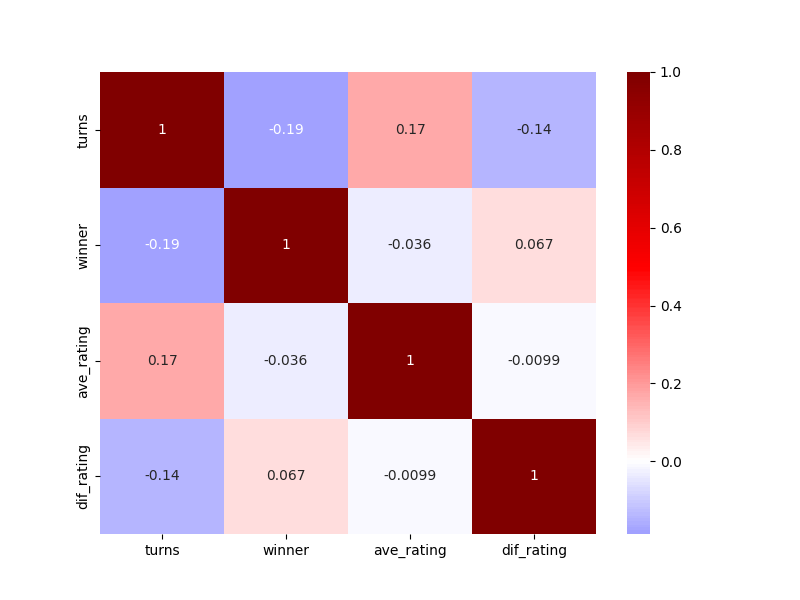
\includegraphics[width=0.8\linewidth]{corr_mat.png}
    \caption{Heat map of the correlation matrix}
    \label{fig:corr_mat}
\end{figure}

\subsection{Connection Between Player Rating and Game Length}
To investigate whether player ratings are associated with game length, we divided players into two groups based on their ratings: those with ratings higher than 1500 (high-rated) and those with ratings lower than 1500 (low-rated). The threshold of 1500 was chosen because it represents the starting rating on the Lichess platform.
\subsubsection*{Mann-Whitney U Test for Game Length}
Since we could not confirm the normality of the rating distribution, we applied the non-parametric Mann-Whitney U test to compare the game lengths between high-rated and low-rated players. Our null hypothesis was that high-rated players' game length mean wasn't higher than low-rated players' mean. The test returned a p-value of \(2.7 \times 10^{-73}\), which allows us to reject the null hypothesis. Therefore, we conclude that player rating significantly influences game length, with higher-rated players tending to play longer games.


\begin{figure}[H]
    \centering
    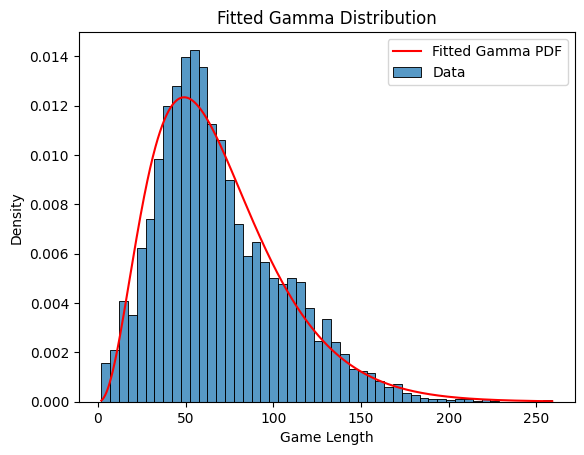
\includegraphics[width=0.8\linewidth]{gamma_fit.png}
    \caption{Gamma distribution estimation of Turns}
    \label{fig:gamma_fit}
\end{figure}
\subsection{Distribution of 'Turns'}

The most comprehensive way to analyze a dataset is through the classification of its distribution. To achieve this, we examine the moments of the distribution for the variable "Turns" as follows:
\[Mean: 61.96255029402662\]
\[Standard Deviation: 33.731730929355365\]
\[Skewness: 0.9052618256476783\]
\[Kurtosis: 1.4921324651335777\]

The kurtosis value (1.5) is higher than expected for a normal distribution, but lower than that of a Poisson distribution, indicating that neither distribution adequately fits the data. The positive skewness (0.9) implies an asymmetric distribution, with a longer tail on the right side.

Given these characteristics, a natural candidate for modeling the data is the Gamma distribution family, known for handling positively skewed data. However, as demonstrated in Figure~\ref{fig:gamma_fit}, the Gamma distribution lacks sufficient flexibility to capture the dataset’s specific shape. To address this limitation, we explored the more general Generalized Gamma distribution, which offers greater shape flexibility.

Despite this improvement, the Generalized Gamma distribution does not sufficiently account for the excess kurtosis. Therefore, we combined it with a Poisson distribution to create a mixture model that captures both the skewness and kurtosis properties. The results of this hybrid model are illustrated in Figure~\ref{fig:gam_poi_fit}.



\begin{figure}[H]
    \centering
    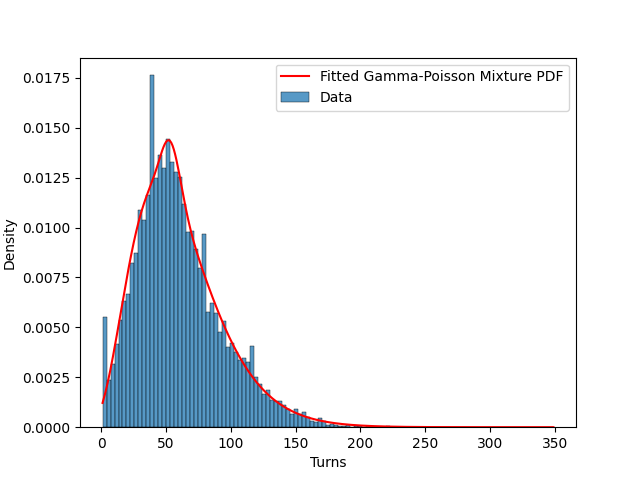
\includegraphics[width=0.8\linewidth]{gamma_poisson_fit.png}
    \caption{Gamma-Poisson distribution estimation of Turns}
    \label{fig:gam_poi_fit}
\end{figure}

\section{Methods}
\subsection{Quantile - Quantile Plot}


\subsection{Kolmogorov-Smirnov Test}
The Kolmogorov-Smirnov (KS) test for normality evaluates whether a sample comes from a normal distribution. It uses the empirical cumulative distribution function (ECDF), $F_n(x)$, of the sample and compares it to the cumulative distribution function (CDF) of the normal distribution, $F(x)$. The test statistic, $D_n$, is defined as:
\[D_n = \sup_x |F_n(x) - F(x)|\]

The null hypothesis $H_0$ assumes that the sample comes from the normal distribution, while the alternative hypothesis $H_1$ posits that it does not.

    If $D_n$ exceeds a critical value (based on the sample size and significance level), we reject $H_0$, concluding the sample deviates significantly from normality.

The KS test is sensitive to both location and shape differences, but less powerful in detecting deviations in the tails of the distribution when compared to other tests like Shapiro-Wilk or Anderson-Darling.
\subsubsection*{2 sample KS test}
Follows the same principles, except it compares two ECDF's from two samples.
\subsection{Correlation Matrix}
A correlation matrix is a table that displays the pairwise correlation coefficients between multiple variables in a dataset. Each element in the matrix represents the degree of linear relationship between two variables, typically measured by Pearson's correlation coefficient:
\[r_{XY} = \frac{Cov(X,Y)}{\sigma_X\sigma_Y}\]

\subsection{Mann-Whitney U Test}
The \textbf{Mann-Whitney U test} is a non-parametric test used to determine whether there is a significant difference between two independent samples. The null hypothesis (\(H_0\)) assumes that the two distributions are identical, and the alternative hypothesis (\(H_a\)) assumes that one distribution tends to have larger or smaller values than the other.


Procedure:

Let \( n_1 \) and \( n_2 \) be the sample sizes of two independent groups, \( X_1, X_2, \dots, X_{n_1} \) and \( Y_1, Y_2, \dots, Y_{n_2} \).

1. Rank all the observations from both groups together, assigning rank 1 to the smallest value, rank 2 to the second smallest, and so on.

2. Compute the sum of the ranks for the first group \( R_1 \).

3. The U statistic for the first group is given by:
\[
U_1 = n_1 n_2 + \frac{n_1(n_1 + 1)}{2} - R_1
\]
Similarly, compute the U statistic for the second group:
\[
U_2 = n_1 n_2 + \frac{n_2(n_2 + 1)}{2} - R_2
\]

4. The Mann-Whitney U statistic is the smaller of \( U_1 \) and \( U_2 \):
\[
U = \min(U_1, U_2)
\]

Normal Approximation (for large samples):

When the sample sizes are large (\(n_1 > 20\) and \(n_2 > 20\)), the distribution of the U statistic can be approximated by a normal distribution with the following mean and standard deviation:

\[
\mu_U = \frac{n_1 n_2}{2}
\]
\[
\sigma_U = \sqrt{\frac{n_1 n_2 (n_1 + n_2 + 1)}{12}}
\]

The standard normal \( Z \)-score is then computed as:
\[
Z = \frac{U - \mu_U}{\sigma_U}
\]

Decision Rule:

To test the null hypothesis, compare the calculated U statistic (or Z-score for large samples) to the critical value from the Mann-Whitney U distribution. If the observed value of \( U \) (or \( Z \)) is extreme enough, reject \( H_0 \) in favor of \( H_a \).

\subsection{Gamma-Poisson distribution}
The GP distribution is a simple average between a general Gamma distribution(GGD) and a Poisson distribution weighted by a parameter w.
\[f_{GP}(x|\alpha, \beta, \gamma, \lambda, w) = wf_{GGD}(x|\alpha, \beta, \gamma) + (1-w)f_P(\lambda)\]
Let us find the MLE of GP:
\[L_{GP}(\alpha, \beta, \gamma, \lambda, w) = \prod_{i=1}^n f_{GP}(x_i|\alpha, \beta, \gamma, \lambda, w)\]
\[= \prod_{i=1}^n [wf_{GGD}(x|\alpha, \beta, \gamma) + (1-w)f_P(\lambda)]\]
Now, by taking the negative log of the likelihood function, we can use minimizing optimization algorithms to find the optimal parameters numerically, since here an analytical solution is difficult to find.

\subsection{Nelder - Mead optimization method}
The Nelder-Mead optimization method is a direct search algorithm used for solving unconstrained nonlinear optimization problems without requiring gradient information. It operates on a simplex, a geometric shape consisting of $n+1$ vertices in an $n$-dimensional space. The algorithm iteratively updates this simplex by reflecting, expanding, contracting, or shrinking its vertices to explore the search space. These transformations aim to minimize an objective function $f(x)$ through comparisons of function values at the simplex vertices. Despite its simplicity, the method is known for efficiency in practice but does not guarantee convergence to a global minimum, especially in higher-dimensional or highly non-convex landscapes. It is widely applied in scenarios where gradient information is unavailable or expensive to compute.


\section{Discussion}

\newpage
\bibliographystyle{IEEEtran}
\bibliography{references}

\end{document}
